\section{What the simulations show}
\label{sec:measured}

This section reports what exact propagation gives for $N=2$--$\num{Nmax_measured}$ and what it implies for the tensor-network cost. Three things are measured: the tunneling signal $\langle\Op\rangle(t)$ (does the cluster oscillate coherently between its two arrangements?), the entanglement entropy across cuts of the particle order (the MPS cut of Section~\ref{sec:fw-tn}, whose entropy sets the bond dimension and hence the cost, Eq.~\eqref{eq:Nstar}), and a correlation graph that describes the entropies and lets them be carried to larger $N$. All numbers are in Table~\ref{tab:measured}; the text discusses what they show. The runs use the correlated start, the mode basis with $k=12$ unless a $k$ is named, and the resonant tilt of each $N$ (Table~\ref{tab:params}, Appendix~\ref{app:numerics}).

\paragraph{What is observed.}
\begin{itemize}[itemsep=0.15em]
\item The signal is a clean oscillation at $N=2,3$ and irregular from $N=4$ on.
\item The central-bond entropy grows with $N$, but by less per added particle than pair counting predicts; the choice of particle order changes it little, and the choice of start changes it a lot.
\item A correlation graph whose edge weights are the one-particle entropy shared among the partners reproduces every measured entropy and rules out the pair-counting law at $N=5,6$.
\item Carried beyond $N=\num{Nmax_measured}$ the graph gives a range of scenarios (Table~\ref{tab:scen}) but no measurement; Section~\ref{sec:static} shows that most of the entropy is present without any tunneling.
\end{itemize}

\subsection{The signal and the cut entropies}
\label{sec:signal}
\label{sec:seed}

\begin{figure}[t]
\centering
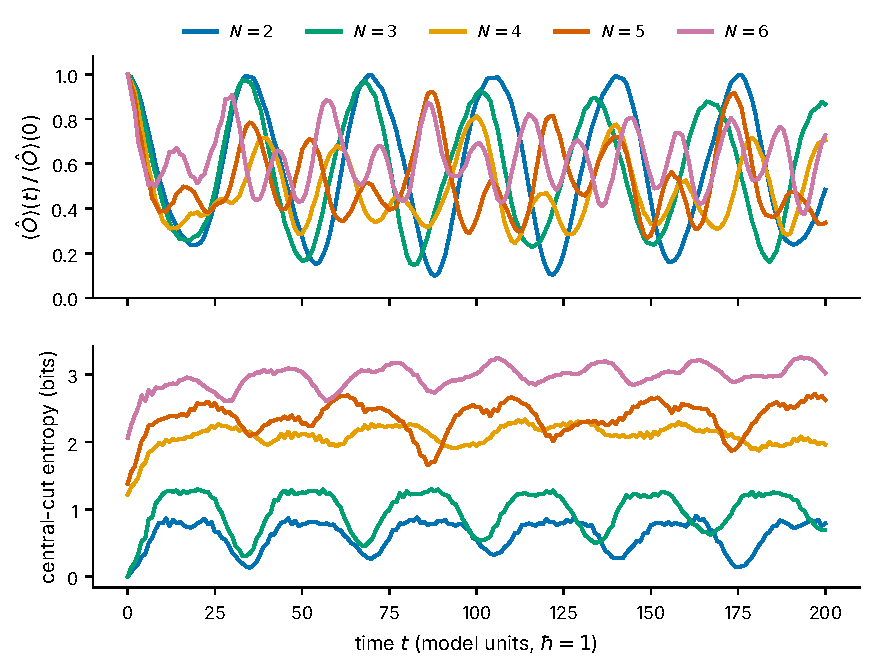
\includegraphics[width=0.78\textwidth]{figures/fig_signal.pdf}
\caption{\textbf{The tunneling signal and its entanglement.} Top: the number of particles in the right valley, normalized to its initial value, for the correlated start at the resonant tilt.
Bottom: entropy across the central bond of the particle order, in bits. Source: the time series stored with each run (Appendix~\ref{app:numerics}).}
\label{fig:signal}
\end{figure}

\begin{table}[!tp]
\centering
\small
\caption{Everything measured on the simulated runs, by cluster size ($k=12$ modes per particle, correlated start at the resonant tilt, one protocol for every $N$: maximum over $[0,T]$ with $T=\num{Tprot}$, snapshot spacing $\num{dtsnap}$; entropies in bits). \emph{Signal} (Fig.~\ref{fig:signal}): lowest value of $\langle\Op\rangle/\langle\Op\rangle(0)$ in the window; largest value after it first falls below $\tfrac12$ (a clean oscillation returns to about one); weight of the start on the gated pair of levels (Table~\ref{tab:start}); time of the central-bond maximum. \emph{Cut entropies} (Eq.~\eqref{eq:threeS}): mean one-particle entropy $\bar S_1$; best balanced, natural-order and worst balanced cut; $\Snat$ is the central bond; numerical Schmidt rank $\chi$ of the central bond at discarded weight $10^{-3}$. \emph{Growth}: increments with each added particle. \emph{Layout}: how much more the worst order pays than the best; how much more the order chosen on the graph pays than the exact optimum; rank correlation between graph and exact costs over all orders. \emph{Graph} (Section~\ref{sec:graph}): mean edge weight $w_{ij}$ against the sharing-law weight $2\bar S_1/(N-1)$ of Eq.~\eqref{eq:sharing}, and the sharing-law central cut against the measured one. \emph{Laws fitted to $N\le4$}: excess of the pair-counting and of the linear law over the measured central bond. \emph{Start}: central bond for the product start (a quench; no run exists for $N\ge5$), to be compared with $\Snat$. A dash marks a quantity that does not exist for that $N$ (an increment, a rank correlation over one order, a fit at the fitted sizes) or a run that was not made.\num{d45_note}}
\label{tab:measured}
\begin{tabular}{lrrrrr}
\toprule
$N$ & 2 & 3 & 4 & 5 & 6 \\
\midrule
\multicolumn{6}{l}{\emph{Signal}} \\
lowest value of $\langle\Op\rangle/\langle\Op\rangle(0)$ & 0.10 & 0.15 & 0.25 & 0.27 & 0.37 \\
largest value after the first fall below $\tfrac12$ & 1.00 & 0.97 & 0.81 & 0.92 & 0.90 \\
weight of the start on the gated pair & 0.98 & 0.94 & 0.46 & 0.35 & 0.31 \\
time of the central-bond maximum & 163 & 89 & 114 & 197 & 193 \\
\multicolumn{6}{l}{\emph{Cut entropies}} \\
$\bar S_1$ & 0.90 & 1.32 & 1.75 & 1.88 & 1.93 \\
best balanced cut $\Sperp$ & 0.90 & 1.29 & 2.33 & 2.62 & 2.88 \\
central bond $\Snat$ & 0.90 & 1.30 & 2.33 & 2.72 & 3.26 \\
worst balanced cut $\Smax$ & 0.90 & 1.37 & 2.54 & 2.93 & 3.70 \\
Schmidt rank $\chi(10^{-3})$ & 7 & 10 & 38 & 74 & 325 \\
$\chi(10^{-3})/2^{\Snat}$ & 3.7 & 4.1 & 7.5 & 11.3 & 34.0 \\
\multicolumn{6}{l}{\emph{Growth}} \\
increment of $\Snat$ & -- & 0.39 & 1.04 & 0.38 & 0.54 \\
increment of $\bar S_1$ & -- & 0.41 & 0.43 & 0.14 & 0.05 \\
\multicolumn{6}{l}{\emph{Layout}} \\
worst order minus best & 0.00 & 0.07 & 0.21 & 0.22 & 0.44 \\
graph-chosen order minus optimum & 0.00 & 0.00 & 0.02 & 0.00 & 0.00 \\
rank correlation, graph against exact & -- & 1.00 & 0.45 & 0.46 & 0.80 \\
\multicolumn{6}{l}{\emph{Graph}} \\
mean edge weight, measured & 1.81 & 1.49 & 1.24 & 1.00 & 0.86 \\
sharing-law weight & 1.81 & 1.32 & 1.16 & 0.94 & 0.77 \\
sharing-law central cut & 0.90 & 1.32 & 2.33 & 2.82 & 3.47 \\
\multicolumn{6}{l}{\emph{Laws fitted to $N\le4$: excess over the measured central bond}} \\
pair-counting law & -- & -- & -- & 0.57 & 1.47 \\
linear law & -- & -- & -- & 0.23 & 0.40 \\
\multicolumn{6}{l}{\emph{Start}} \\
central bond, product start (correlated start: $\Snat$ above) & 0.90 & 2.31 & 4.81 & -- & -- \\
\bottomrule
\end{tabular}
\end{table}


\paragraph{Signal.} At $N=2,3$ the observable falls to a small fraction of its initial value and returns almost completely: a clean oscillation of one particle between the valleys at a single splitting. From $N=4$ the lowest value is higher, the return is incomplete and the curves become irregular (Fig.~\ref{fig:signal}). The weight of the start on the gated pair of levels, the pair of smallest splitting that passes the doublet gates, drops with it; it measures the pair selector and the basis as much as the cluster, and the two levels that actually carry the weight give a different picture (Section~\ref{sec:static}). Where a clean doublet exists the ratio $g_N=\dE_2/\dE_N$ of Eq.~\eqref{eq:Tobs} lies between $\num{gN_lo}$ and $\num{gN_hi}$, which supports carrying $g_N=1$ in the quantum price; where it does not, the first minimum of $\langle\Op\rangle(t)$ defines $\Tobs$. The central-cut entropy rises within the first period and then oscillates; its maximum lies inside every window, but late at $N=2,5,6$, where it keeps creeping up with the window (Table~\ref{tab:protocol}).

\paragraph{Growth is not constant per particle.} The central bond grows unevenly, and by less per particle than pair counting predicts. The largest step is the one into $N=4$, the first size at which the $k=12$ basis does not hold a clean doublet (Table~\ref{tab:start}); how much of it belongs to the cluster and how much to the basis is not settled. The one-particle entropy saturates quickly, so the growth of the central bond is carried by the number of partners rather than by the entropy of each particle. The constant-growth law (Eq.~\eqref{eq:HS}) and the pair-counting law (Eq.~\eqref{eq:HP}) each have two parameters and can be made to pass through the points $N\le4$; they then disagree with each other and with the data at $N=5$ and $N=6$.

\paragraph{The layout matters little.} The best balanced cut $\Sperp$, the natural-order cut $\Snat$ and the worst balanced cut $\Smax$ differ by a small amount that grows with $N$. The natural order is among the best of all $N!/2$ orders at $N=3,\dots,6$, so $\SN=\Snat$ is the conservative-for-the-classical-side reading: the best order is already used.

\paragraph{The start matters a lot.} The product start ignores the correlation hole of particles that share a valley, so it is a quench that injects entropy, far above that of the correlated start already at $N=3,4$. Charging it would inflate the classical cost by a factor that grows with $N$; we use the correlated start, which is also the physical isomer.

\paragraph{Basis and compression.} The central entropy falls with $k$ at $N=4,5$, while the numerical Schmidt rank at discarded weight $10^{-3}$ rises (Table~\ref{tab:k}, Appendix~\ref{app:numerics}). The rank is far above $2^{S}$ and the ratio grows with $N$, so a matrix-product state that stores the state to this accuracy is more expensive than the $\chi=2^S$ of the cost model (Section~\ref{sec:walls}). Neither quantity is converged in $k$.

\subsection{The cut entropy is a cut of a correlation graph}
\label{sec:graph}

The entropies of Table~\ref{tab:measured} are well described by a graph on the particles whose edge weights are measured mutual informations.

\paragraph{The graph.}
Idea: the entropy across a cut is large when many particles on one side are strongly correlated with particles on the other. If we know how correlated each pair is, we can add up the correlation across the cut instead of computing the full entropy, and we can search for the particle order whose worst cut is cheapest. Quantitatively, let $I_{ij}(t)=S_i+S_j-S_{ij}$ be the mutual information (bits) between particles $i$ and $j$ and $w_{ij}=\max_tI_{ij}(t)$. For a pure state $S_A=\tfrac12I(A\!:\!A^c)$, so the natural estimate of the entropy across $A\,|\,A^c$ is
the weight of the cut edges,
\begin{equation}
C(A)=\tfrac12\sum_{i\in A,\ j\notin A}w_{ij}.
\label{eq:Cgraph}
\end{equation}
Choosing a matrix-product order is then choosing a linear order of the vertices that keeps the maximal prefix cut small (a weighted cutwidth), and choosing a tree is a carving problem (tree structures can also be optimized automatically from the measured entanglement~\cite{hikihara2023}); a balanced minimum cut is the lower bound that every layout pays and a balanced
maximum cut is the worst layout. Mutual-information graphs have been used to \emph{choose} the orbital order of density-matrix renormalization group
calculations~\cite{rissler2006,barcza2011,szalay2015}; the idea of reading an entropy as a cut is not new. For classical networks the maximum flow equals the minimum cut~\cite{dantzig2003max}; in continuum geometries the largest flux of a divergenceless vector field of bounded norm equals the area of a minimal surface (flow--cut theorems~\cite{headrick2018riemannian}), which is the content of the bit-thread picture of holographic entanglement entropy~\cite{freedman2017}. Entropy equals a minimum cut in random tensor networks~\cite{hayden2016,fitter2025}, which Ref.~\cite{fitter2025} treats as a max-flow problem, and for graph states it is the rank of the cut adjacency matrix~\cite{hein2004}; flows and cuts of entanglement are also used for entanglement distribution in quantum networks~\cite{yang2022strong}.
For general tensor networks the quantum max-flow and min-cut can differ~\cite{cui2016,gesmundo2018}, so a cut count bounds the entropy only in specific settings. Our $C(A)$ uses none of this machinery: it is a pairwise estimator on a graph of measured mutual informations, not a tensor-network cut, and it is tested against the exact entropy.

\paragraph{What is exact and what is not.}
Three pairwise statements are exact (Proposition~\ref{prop:graph}, Appendix~\ref{app:proofs}): for $|A|=2$, $S_A=S_i+S_j-I_{ij}$; for any spanning tree $\tau$ of $A$, $S_A\le\sum_{i\in A}S_i-\sum_{\tau}I_{ij}$ (the entropy analogue of the Chow--Liu tree approximation~\cite{chowliu1968}); and at $N=3$
and fixed $t$, $C(\{i\})=S_i$. The general statement is not: pairwise mutual information is neither an upper nor a lower bound on $S_A$ (a GHZ-type state overcounts, a scrambled state undercounts). The sum $\sum_jI_{ij}\le2S_i$ would follow from monogamy of
mutual information, which holds for holographic states~\cite{hayden2013} but not in general (a GHZ state, which is a stabilizer state, violates it). We therefore test Eq.~\eqref{eq:Cgraph} on the data.

\begin{figure}[t]
\centering
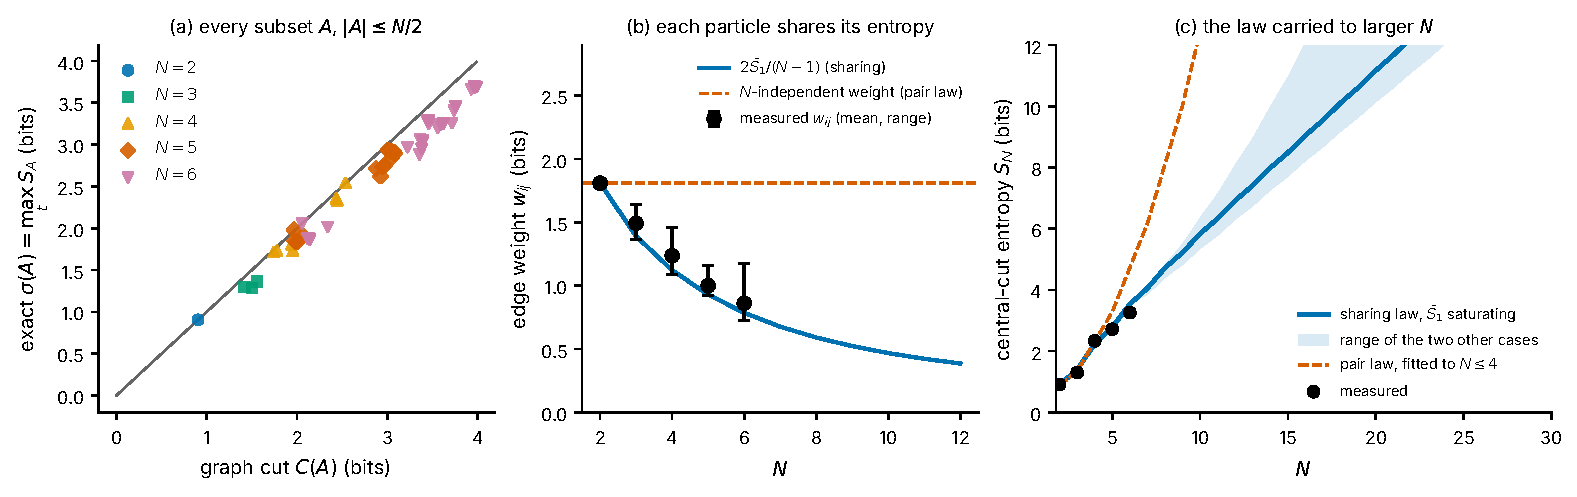
\includegraphics[width=\textwidth]{figures/fig_entropy.pdf}
\caption{\textbf{The graph explains the entropy, and why its growth falls.} (a) Exact $\sigma(A)=\max_tS_A$ against the graph cut $C(A)$ for every subset with $|A|\le N/2$ at $N\le6$. (b) Mean edge weight $w_{ij}$ with its range, against the sharing
law $2\bar S_1/(N-1)$ and against the $N$-independent weight that the pair-counting law assumes. (c) Central-cut entropy against $N$: measured (black), the pair law fitted to $N\le4$ (dashed), and the sharing law carried to larger $N$ (Section~\ref{sec:larger}); shading spans the other two
scenarios for the one-particle entropy. Computed from the stored time series of each run (Appendix~\ref{app:numerics}).}
\label{fig:entropy}
\end{figure}

\paragraph{Test.} The graph reproduces the entropy of every subset at $N\le6$ (Fig.~\ref{fig:entropy}a): it overestimates the exact entropy by up to $\num{graph_maxdev}$ bit ($N=6$) and underestimates it by at most $\num{graph_maxunder}$ bit. The overcount at $N=3$ is a property of the time maxima: at fixed $t$ the graph is exact there, but the maximum over $t$ of each edge occurs at different times. The graph is also a good guide to the layout: the order that minimizes the maximal prefix cut on the graph costs at most a few hundredths of a bit more than the exact optimum, and the rank correlation between graph and exact costs is high at $N=3,6$ and modest at $N=4,5$ (Table~\ref{tab:measured}). It finds a near-best order but ranks the rest unreliably there.

\paragraph{Why the growth falls: each particle shares a finite entropy (a description, not a derivation).}
The measured edge weights are nearly uniform within each $N$ and fall with $N$ (Fig.~\ref{fig:entropy}b, Table~\ref{tab:measured}). In a pure state a particle's entropy is the mutual information it shares with all the others, $\sum_jI_{ij}\approx2S_i$; the measured ratio is between $\num{mono_lo}$ and $\num{mono_hi}$ for all $N$ and $i$. The sum rule is an identity only when monogamy holds, and a finite entropy does not by itself force equal weights (a state can concentrate it on a few partners); we use the near-equality as an observation. In words: each particle has a finite amount of entanglement to give, and the more partners there are, the thinner each share. If each particle spreads its entropy evenly over its $N-1$ partners,
\begin{equation}
w_{ij}\simeq\frac{2\bar S_1}{N-1},\qquad
S_N\simeq C(\{1..b\})=\frac{b(N-b)}{N-1}\,\bar S_1(N),\quad b=\lfloor N/2\rfloor,
\label{eq:sharing}
\end{equation}
where $\bar S_1$ is the mean one-particle entropy and the prefactor is $\simeq(N+1)/4$. The law reproduces the measured weights and central cuts; at $N=5,6$ the cut it gives lies inside the layout bracket, as a size-class average should (Lemma~\ref{lem:chord}), and above the natural-order cut. The pair-counting law is the opposite assumption, an $N$-independent weight on each of the $\lfloor N/2\rfloor\lceil N/2\rceil$ crossing pairs. A particle cannot give every one of a growing number of partners the same entropy, and the data show it does not: fitted to $N\le4$ the pair law overshoots at $N=5$ and $N=6$ by more than the spread of layouts and lies above even the worst layout, and the linear law fitted the same way is high by an amount comparable to that spread (Table~\ref{tab:measured}, Table~\ref{tab:scen}).

\paragraph{Why the shares thin out.} The saturation of $\bar S_1$ and the $1/(N-1)$ fall of the shares are what a monogamy relation for mutual information describes: if one particle has a bounded entanglement capacity, the share it gives to each partner must fall as the number of partners grows~\cite{hayden2013}. The measured sum rule sits at the boundary of that relation, where the sharing law is exact, and a similar dilution of orbital mutual information among many partners is seen in correlation graphs of molecules~\cite{rissler2006,barcza2011}. Monogamy of mutual information is not a general property (above), so this is a consistency argument, not a derivation. With the shares thin, the central cut grows as $b(N-b)/(N-1)\simeq N/4$ times $\bar S_1$, that is linearly in $N$ once $\bar S_1$ has saturated, and not as the $b(N-b)\sim N^2/4$ of the pair-counting law. This is the growth that decides the cost of a matrix-product state, whose bond dimension is bounded below by the exponential of the cut entropy~\cite{schuch2008}. What the data support is the rejection of the pair law at $N=6$; they do not yet separate the sharing law from other linear growth.

\begin{figure}[t]
\centering
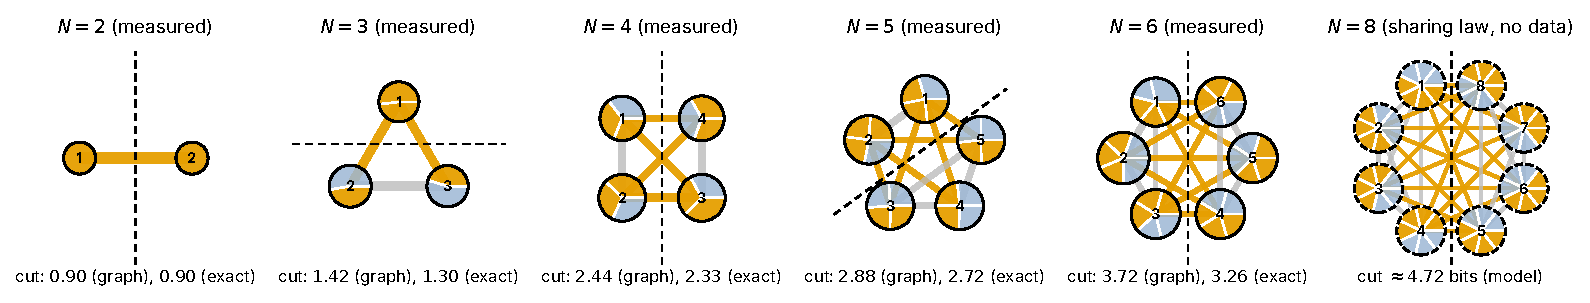
\includegraphics[width=\textwidth]{figures/fig_venn.pdf}
\caption{\textbf{Adding particles to the correlation graph.} Each disk is a particle; its area is the entropy it shares, $\sum_jw_{ij}/2$, on the same scale in every panel. A disk is divided into one petal per partner (angle proportional to $w_{ij}$),
and the petals of $i$ and $j$ are joined by a ribbon of width proportional to $w_{ij}$. The dashed line is the central cut: orange ribbons cross it, and the entropy across the cut is their total width ($C$ in the caption of each panel; exact value for comparison). Adding a particle
adds a disk and $N$ ribbons, but the old disks cannot grow much, so every petal, and every ribbon, thins; the number of crossing ribbons grows as $b(N-b)$. The panel at $N=8$ is drawn from the sharing law, not from data (dashed outlines).}
\label{fig:venn}
\end{figure}

Fig.~\ref{fig:venn} draws this. Going from $N=2$ to $5$ the graph gains disks and ribbons that cross the cut, and each ribbon becomes thinner; the net growth of the cut is the product of the two.


\paragraph{What is not established.}
\begin{itemize}[itemsep=0.15em]
\item Eq.~\eqref{eq:Cgraph} is validated on $N\le6$ only. It is an estimator and a layout heuristic, not a bound, and with time-maximal weights it overcounts.
\item Eq.~\eqref{eq:sharing} assumes that each particle shares its entropy evenly with its partners and that the graph stays dense; the data are consistent with the first, and the second may fail for large, spatially extended clusters.
\item The graph cannot say whether $\bar S_1$ saturates beyond $N=6$. That is the one input of the extrapolation below.
\end{itemize}


\subsection{\texorpdfstring{Carried to larger $N$}{Carried to larger N}}
\label{sec:larger}

Eq.~\eqref{eq:sharing} turns the question ``how does $\SN$ grow?'' into ``how does $\bar S_1(N)$ behave?''. The one-particle entropy is bounded (by $\log_2k$ at fixed $k$) and its measured increments shrink from $N=3$ on (Table~\ref{tab:measured}). We carry it forward in three stated scenarios, none of which is a measurement beyond $N=\num{Nmax_measured}$ (parameters and extrapolated values in Table~\ref{tab:scen}):
\begin{itemize}[itemsep=0.15em]
\item \emph{saturating (fit):} $\bar S_1(N)=S_\infty-(S_\infty-\bar S_1(2))e^{-(N-2)/\tau}$ with two parameters fitted to the measured values and anchored at $N=2$;
\item \emph{saturated at $N=\num{Nmax_measured}$:} $\bar S_1$ stays at its last measured value, the earliest saturation the data allow (the optimistic case for the classical side);
\item \emph{keeps growing:} $\bar S_1$ grows by the mean of the last two measured increments per particle (the pessimistic case for the classical side; the central cut then grows as $N^2$).
\end{itemize}
In the first two cases $\SN$ is asymptotically linear with slope $\bar S_1^\infty/4$ per added particle. Fig.~\ref{fig:entropy}c shows the three curves against the pair law.

\begin{table}[ht]
\centering
\small
\caption{The three scenarios for the one-particle entropy $\bar S_1(N)$ beyond the simulated sizes, the growth laws fitted to smaller $N$, and what they predicted for the central bond (bits). The sharing-law rows were fitted to $N\le5$ and give the central cut they predicted at $N=6$ before that run, and its excess over the measured $S_6=\num{S6_cen}$; the pair-counting and linear laws were fitted to $N\le4$. \emph{Slope}: asymptotic growth per added particle (the sharing law with saturating $\bar S_1$ is linear in $N$; with growing $\bar S_1$ it grows as $N^2$). The last three columns are the extrapolated central bond. None of these is a measurement beyond $N=\num{Nmax_measured}$.}
\label{tab:scen}
\begin{tabular}{llcccccc}
\toprule
scenario & parameters & slope & $N=6$ & excess & $N=8$ & $N=12$ & $N=16$ \\
\midrule
sharing, $\bar S_1$ saturating (fit) & $S_\infty=\num{fit_Sinf}$, $\tau=\num{fit_tau}$ & 0.53 & 3.71 & 0.46 & 4.72 & 6.92 & 9.05 \\
sharing, $\bar S_1$ saturated at $N=6$ & $\bar S_1=\num{S1_last}$ & 0.48 & 3.39 & 0.13 & 4.41 & 6.31 & 8.22 \\
sharing, $\bar S_1$ keeps growing & $+\num{inc_pess}$ per particle & $\propto N^2$ & 3.90 & 0.64 & 4.82 & 8.08 & 12.07 \\
pair-counting law & fit to $N\le4$ & $\propto N^2$ & 4.73 & 1.47 & 8.11 & 17.76 & 31.27 \\
linear law & fit to $N\le4$ & 0.71 & 3.66 & 0.40 & 5.09 & 7.95 & 10.81 \\
\bottomrule
\end{tabular}
\end{table}



\paragraph{The $N=6$ comparison.} The sharing law fitted to $N\le5$ and the pair and linear laws fitted to $N\le4$ give predictions for the central bond at $N=6$ (Table~\ref{tab:scen}), which the simulation at $N=6$ ($S_6=\num{S6_cen}$ bit, $k=12$) tests. It decides against the pair law, which is too high and above even the worst layout. It does not vindicate the sharing law as a predictor: all three scenarios overshoot, and so does the linear law. The assumption behind the scenarios holds, since the one-particle entropy grows by very little, and the sharing law fed with the measured $\bar S_1$ gives a value inside the layout bracket (Table~\ref{tab:measured}). What it overstates is the prefactor: the natural-order bond lies below the size-class average, as it does, by less, at $N=5$. The curves of the three scenarios are refitted through the $N=6$ point, so the walls of Section~\ref{sec:walls} use $N\le6$. One further point cannot separate the sharing law from linear growth: the measured step is close to the asymptotic slope of the sharing law.

The prefactor can also be tested on the stored runs. Fed with each run's own $\bar S_1$, the sharing law reproduces the measured central entropy of all correlated-start runs ($N=2$--$\num{shr_Nmax}$, every stored $k$) to within a measured-to-law ratio of $\num{shr_lo}$--$\num{shr_hi}$, so the small overshoot is a property of the correlated start across $N$ and $k$, not of one run. The product start, a quench, does not follow the law at $N=4$, $k=12$ (ratio $\num{shr_prod_N4}$); at $N=3$ it still holds, with a much larger $\bar S_1$.

\FloatBarrier
